\documentclass[12pt,a4paper]{article}
\usepackage[margin=0.5in]{geometry}

\usepackage{polski}
\usepackage[utf8]{inputenc}

\usepackage{graphicx}
\usepackage{float}
\usepackage{setspace} %texlive-latex-recommended
\usepackage{enumitem}

\usepackage{tabularx}

\newcommand{\imgz}{0.44\linewidth}
\newcommand{\numerzajec}{4}
\newcommand{\tematzajec}{Przeszukiwanie labiryntu.}
\newcommand{\datazajec}{30 maja 2017}


\begin{document}
	\thispagestyle{empty}
	\begin{center}
		\vspace*{1.6cm}
		
\includegraphics[width=0.55\linewidth]{obrazki/pblogo.png}	\\
		\vspace{0.5cm}
		\large
		\textsf{\textbf{Sprawozdanie z pracowni specjalistycznej}} \\
		\vspace{0.5cm}
		\textsf{\textbf{\textit{Sztuczna inteligencja}}}	\\
		\vspace{1cm}
		\textsf{Projekt numer: \textbf{\numerzajec}}	\\
		\vspace{0.5cm}
		\textsf{Temat: \textbf{\tematzajec}}
	\end{center}

	\vspace{2cm}
	\begin{tabular}{rl}
        Wykonujący ćwiczenie: &\textbf{Tobiasz Dzieszkowski} \\
                              & \textbf{Adrian Kryński} \\
                              & \textbf{Karol Budlewski} \\
	\end{tabular}

	\vspace{3.5cm}	

	\begin{minipage}{0.45\linewidth}
		\large
		\begin{spacing}{1.5}
		Studia dzienne \\
		Kierunek: Informatyka \\
		Semestr: IV \\
		\end{spacing}
	\end{minipage}
	\begin{minipage}[t]{0.5\linewidth}
		\large
		\begin{spacing}{1.2}
		Grupa zajęciowa: PS4
		\end{spacing}
	\end{minipage}
	
	Prowadzący ćwiczenie: \textbf{mgr inż. Michał Czołombitko} \\
	
	\begin{flushright}
		\begin{minipage}[t]{0.3\linewidth}
			\centering
			................. \\
			\small OCENA
		\end{minipage}
	\end{flushright}
	
	\begin{minipage}[t]{0.4\linewidth}
		\centering
		Data \\
		\small \datazajec
	\end{minipage}
	
	\begin{flushright}
		\begin{minipage}[t]{0.5\linewidth}
			\centering
			............................................. \\
			\small \textsf{Data i podpis prowadzącego}
		\end{minipage}
	\end{flushright}
	\pagebreak
	%%%%%%%%%%%%%%%%%%%%%%%%%%%%%%%%%%%%%%%%%%%%%%%%%

	\tableofcontents

	\pagebreak
	%%%%%%%%%%%%%%%%%%%%%%%%%%%%%%%%%%%%%%%%%%%%%%%%%

	
	\section{Wstęp}
	Celem projektu było stworzenie aplikacji wykorzystującej różne
	strategie przeszukiwania do znajdowania wyjścia z labiryntu, oraz
	zwizualizowanie ich działania.
	
	Efektem końcowym jest aplikacja pozwalająca na przechodzenie
	labiryntu. Udostępnia ona kilka różnych algorytmów, między innymi
	przeszukiwanie w głąb oraz przeszukiwanie wszerz. Dodatkowo oferuje
	przystępny interfejs tworzenia labiryntu, z którym każdy będzie w
	stanie stworzyć idealną dla siebie strukturę. Aplikacja pozwala
	również zapis swojego labiryntu oraz jego późniejsze wczytanie.
	
	\section{Wymagania systemowe}
		\begin{enumerate}[label=•]
			\item System operacyjny: dowolny system operacyjny ze 
				wsparciem dla Qt 5 (np. Windows 10, Ubuntu, Gentoo, 
				MacOS)
			\item Procesor: Amd Athlon 64 lub nowszy
			\item Pamięć RAM: 2 GB
			\item Karta graficzna: dowolna karta graficzna wspierająca
				OpenGL 2.1 lub DirectX 11 (Windows)
			\item Dysk twardy: minimum 100 MB wolnego miejsca
			\item Dodatkowe: obsługa myszki
		\end{enumerate}
		
	\section{Interfejs użytkownika}
	
	\begin{figure}[H]
		\centering
		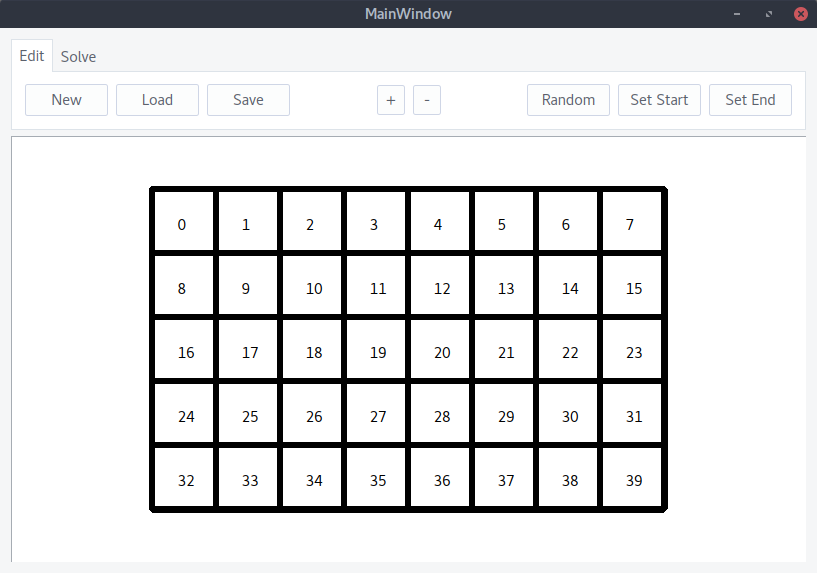
\includegraphics[width=0.8\linewidth]{obrazki/1.png}
		\caption{Tmp}
	\end{figure}
	
	\begin{figure}[H]
		\centering
		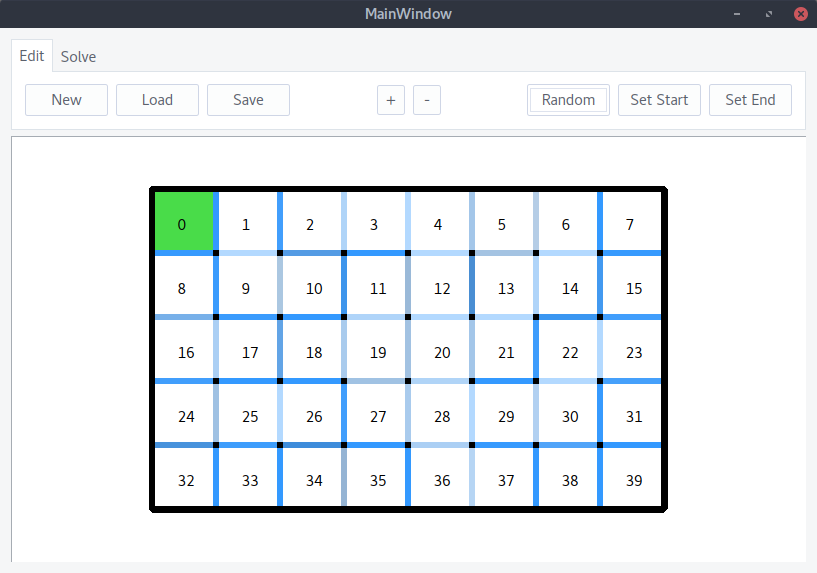
\includegraphics[width=0.8\linewidth]{obrazki/2.png}
		\caption{Tmp}
	\end{figure}
	
	\begin{figure}[H]
		\centering
		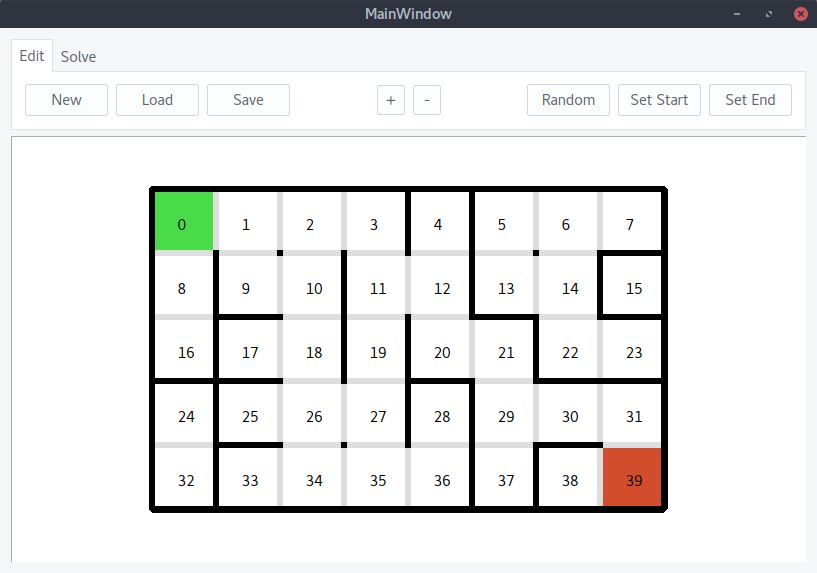
\includegraphics[width=0.8\linewidth]{obrazki/4.png}
		\caption{Tmp}
	\end{figure}
	
	\begin{figure}[H]
		\centering
		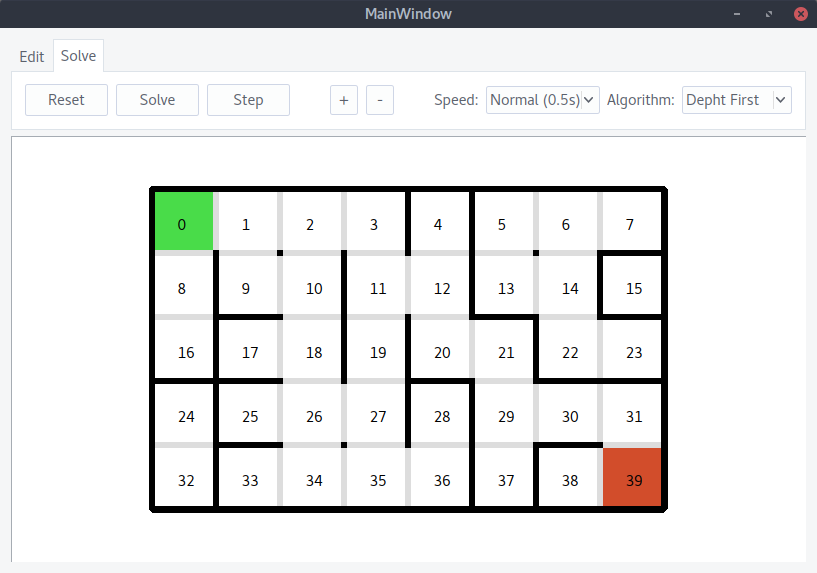
\includegraphics[width=0.8\linewidth]{obrazki/5.png}
		\caption{Tmp}
	\end{figure}
	
	\begin{figure}[H]
		\centering
		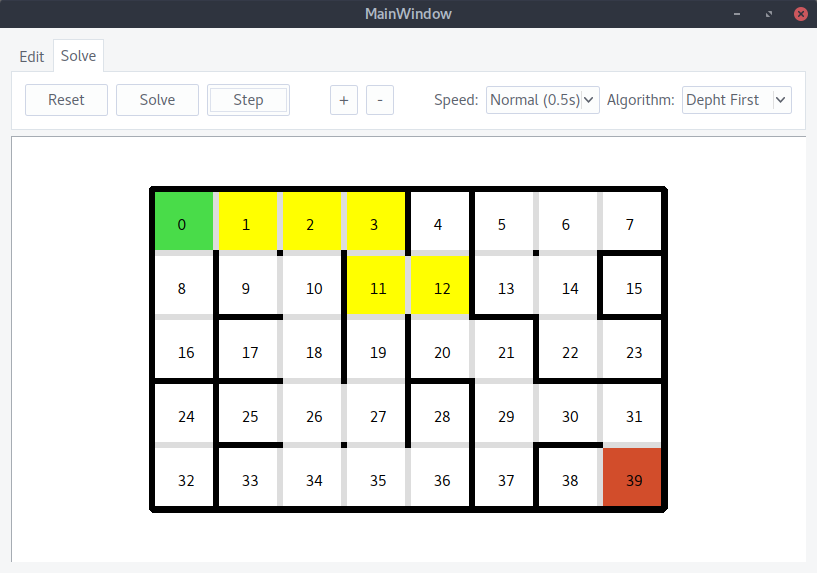
\includegraphics[width=0.8\linewidth]{obrazki/6.png}
		\caption{Tmp}
	\end{figure}
	
	\begin{figure}[H]
		\centering
		
\includegraphics[width=0.8\linewidth]{obrazki/7i8.png}
		\caption{Tmp}
	\end{figure}
	
	\begin{figure}[H]
		\centering
		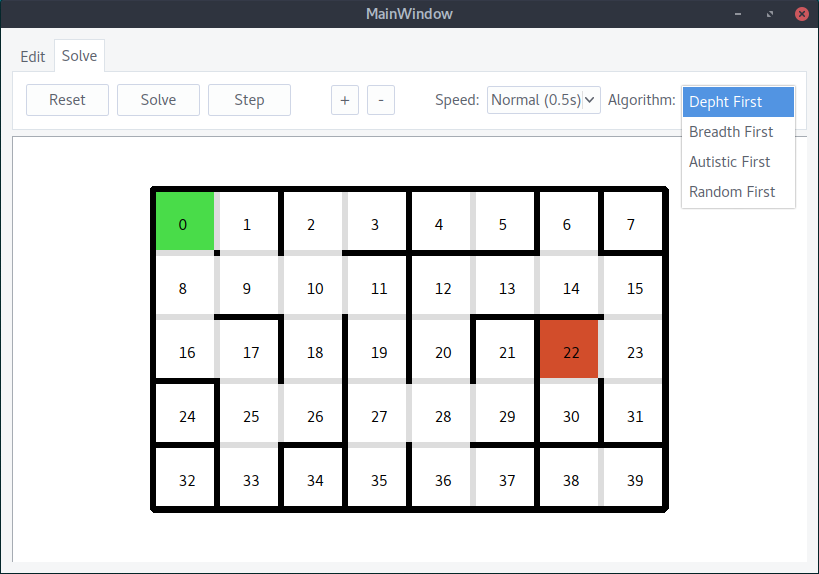
\includegraphics[width=0.8\linewidth]{obrazki/9_new.png}
		\caption{Tmp}
	\end{figure}
	
	\begin{figure}[H]
		\centering
		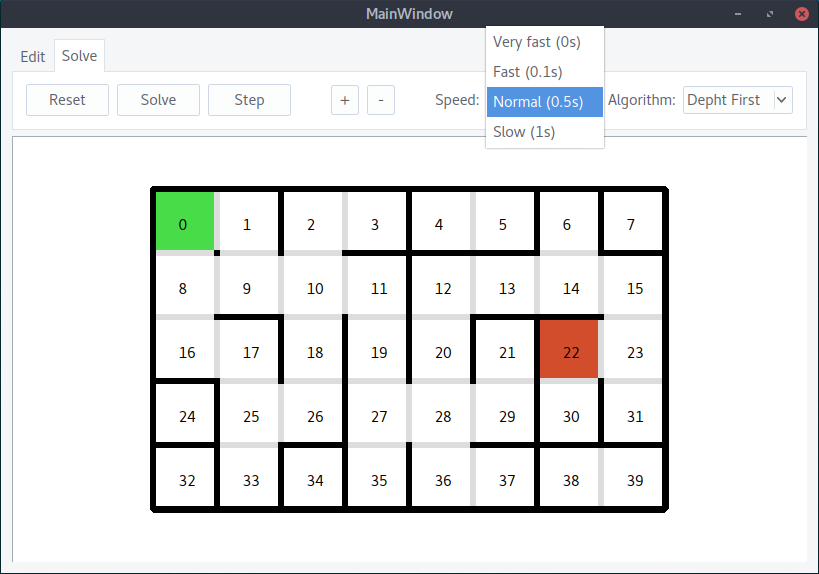
\includegraphics[width=0.8\linewidth]{obrazki/10_new.png}
		\caption{Tmp}
	\end{figure}
	
	\begin{figure}[H]
		\centering
		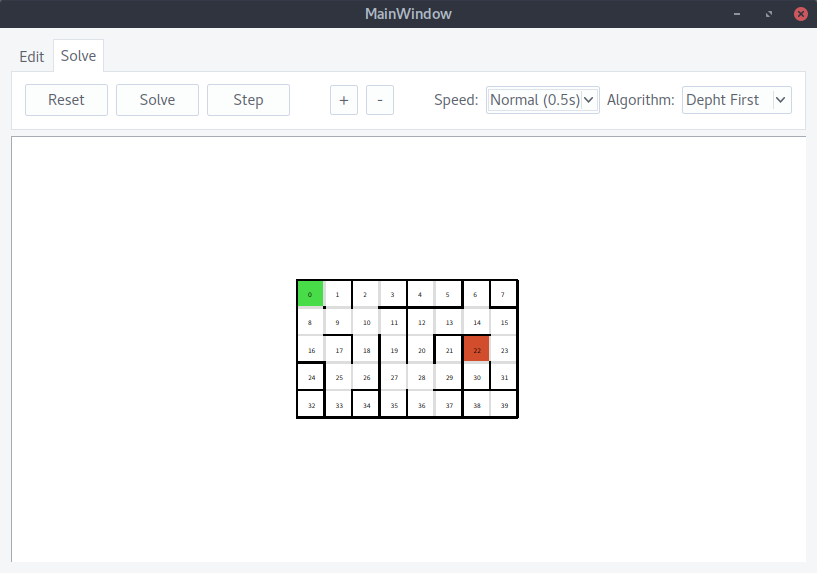
\includegraphics[width=0.8\linewidth]{obrazki/11.png}
		\caption{Tmp}
	\end{figure}
	
	\begin{figure}[H]
		\centering
		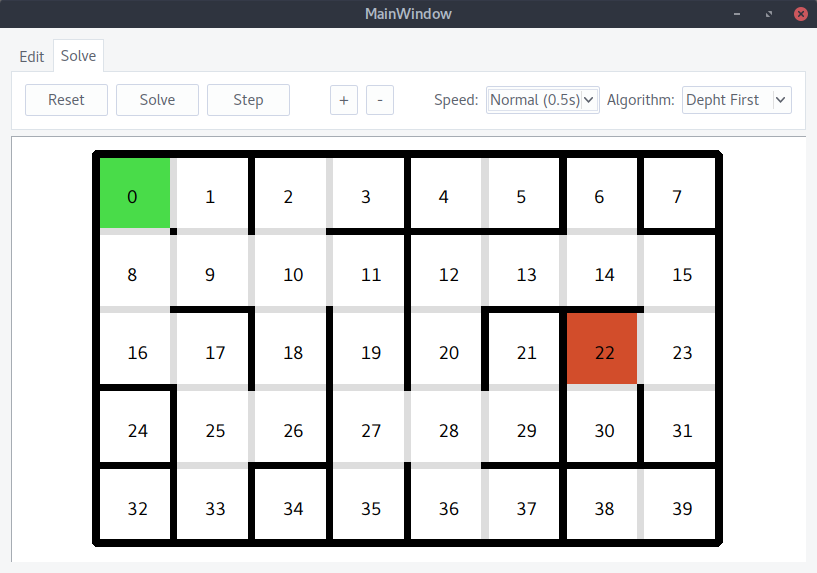
\includegraphics[width=0.8\linewidth]{obrazki/12.png}
		\caption{Tmp}
	\end{figure}
	
	\begin{figure}[H]
		\centering
		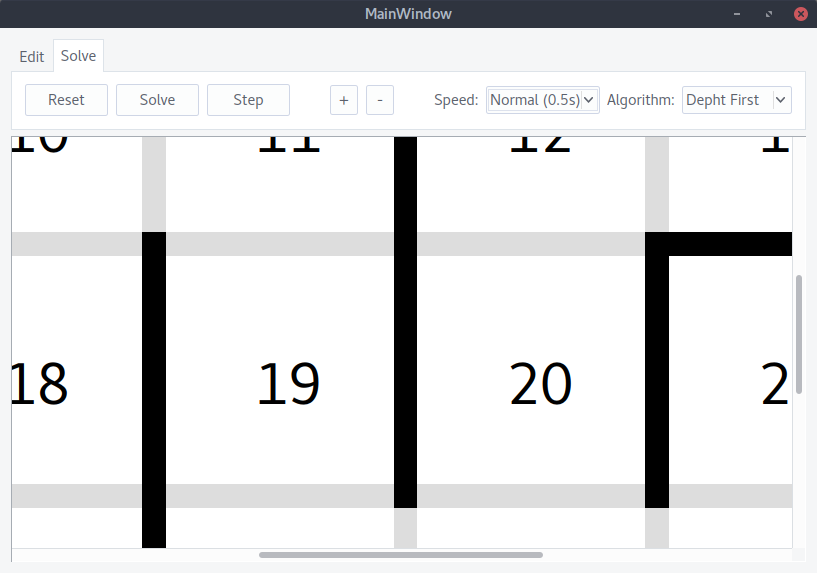
\includegraphics[width=0.8\linewidth]{obrazki/13.png}
		\caption{Tmp}
	\end{figure}
	
	\begin{figure}[H]
		\centering
		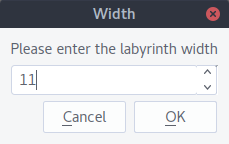
\includegraphics[width=0.8\linewidth]{obrazki/14.png}
		\caption{Tmp}
	\end{figure}
	
	\begin{figure}[H]
		\centering
		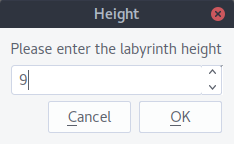
\includegraphics[width=0.8\linewidth]{obrazki/15.png}
		\caption{Tmp}
	\end{figure}
	
	\begin{figure}[H]
		\centering
		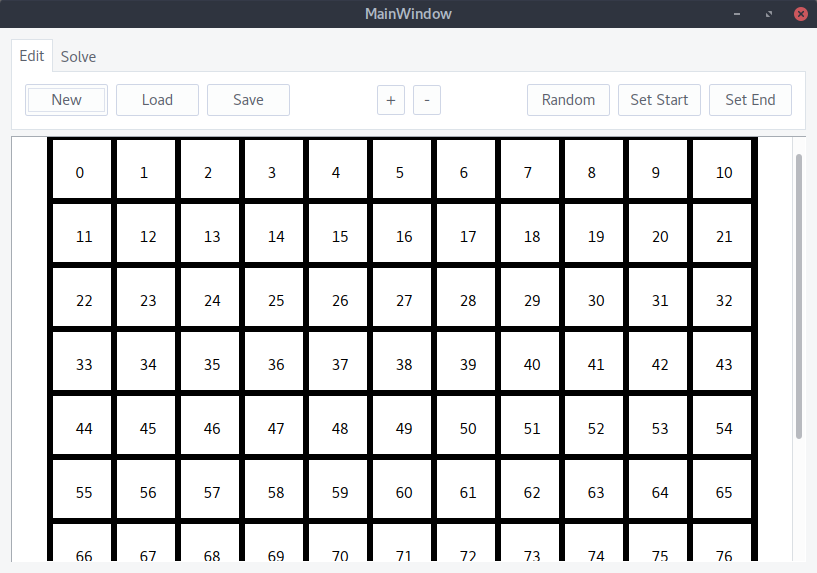
\includegraphics[width=0.8\linewidth]{obrazki/16.png}
		\caption{Tmp}
	\end{figure}
	
	\section{Strategie przeszukiwania}
	\subsection{Przeszukiwanie w głąb (DFS, Depth First)}
	Algorytm działa następująco: jeśli ma możliwość pójścia dalej,
	preferuje pola w kolejności: lewo, góra, prawo, dół. Następnie 
	przechodzi do wybranego pola i ponownie wybiera preferowane pole. 
	Będzie on powtarzał te czynności do momentu odnalezienia 
	pola końcowego lub do znalezienia się w ślepym zaułku. W takim	
	wypadku cofa się do poprzedniego pola i sprawdza czy może pójść w 
	inną stronę. Jeżeli nie - znowu się cofa. W przypadku braku
	drogi do pola końcowego algorytm cofnie się na sam początek i
	zakończy działanie. \textbf{Nie znajduje on najkrótszej ścieżki.}
	
	\subsection{Przeszukiwanie wszerz (BFS, Breadth First)}
	Algorytm działa następująco: w pętli dodaje wszystkich sąsiadów 
	bieżącego pola do kolejki odwiedzając każde z nich oraz ustawia 
	dla nich poprzednika. Następnie bierze pierwsze pole czekające w 
	kolejce i wykonuje to samo. Wykonuje te czynności dopóki nie 
	znajdzie pola końcowego lub wszystkie pola zostaną ozanczone jako 
	odwiedzone.
	\textbf{Znajduje on najkrótszą ścieżkę.}
	
	\subsection{Przeszukiwanie losowe (Random First)}
	Algorytm działa następująco: wybiera losowe sąsiadujące pole, a
	następnie do niego przechodzi. Powtarza tę czynność do momentu
	odnalezienia pola końcowego lub znalezienia się w ślepym zaułku. W 
	takim wypadku cofa się do poprzedniego pola i sprawdza czy może
	pójść w inną (losową) stronę. Jeżeli nie - znowu się cofa. W 
	przypadku braku drogi do pola końcowego algorytm cofnie się na sam 
	początek i zakończy działanie. \textbf{Nie znajduje on najkrótszej 
	ścieżki.}
	
	\section{Budowanie ze źródeł}



\end{document}
